\section{Method}
\label{sec:method}
% defines commands used below to insert datastructure (for better readability)
\newcommand{\formalcontexttable}{%
\begin{table}[]
\centering
\caption{Formal context}
\label{tab:formal_context}
\begin{tabular}{|l|c|c|c|c|c|}
\hline
          & $x_A$           & $x_B$           & $x_C$           & $x_D$           & \dots \\ \hline
$c_1$         & $\times$    & $\times$    &             &             &        \\ \hline
$c_2$         &             &             & $\times$    & $\times$    &        \\ \hline
$c_1 \vee c_2$ & $\times$    & $\times$    & $\times$    & $\times$    &        \\ \hline
$\vdots$      &             &             &             &             & $\ddots$ \\ \hline
\end{tabular}%
\end{table}%
}

\newcommand{\dendogram}{%
\begin{figure}[]
\centering
\caption{Dendrogram with objects on the bottom.}
\label{fig:dendrogram}

\begin{tikzpicture}[scale=1]
% Positions of objects (bottom)
\node (A) at (0,0) {$x_A$};
\node (B) at (2,0) {$x_B$};
\node (C) at (4,0) {$x_C$};
\node (D) at (6,0) {$x_D$};

% Merge A and B
\coordinate (ABtop) at (1,1);
\draw (A) -- (0,1) -- (ABtop) -- (2,1) -- (B);

% Merge C and D
\coordinate (CDtop) at (5,1);
\draw (C) -- (4,1) -- (CDtop) -- (6,1) -- (D);

% Merge AB and CD
\coordinate (root) at (3,2);
\draw (ABtop) --(1,2) -- (5,2) -- (CDtop);

\end{tikzpicture}
\end{figure}
}

\newcommand{\lattice}{%
\begin{figure}[h]
\centering
\caption{Concept lattice for the transposed formal context.}
\label{fig:concept_lattice}

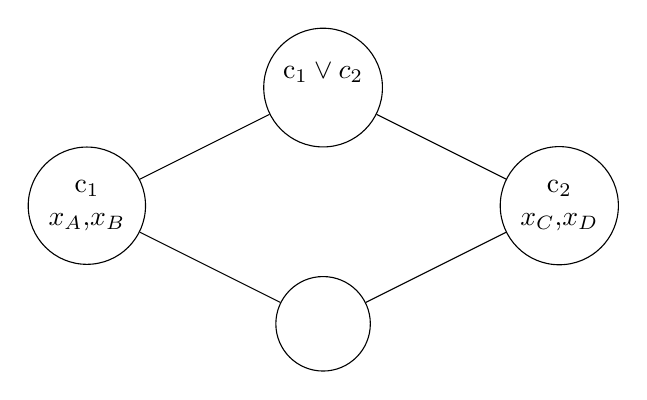
\begin{tikzpicture}[scale=1, every node/.style={draw, circle, align=center, minimum width=1.2cm, minimum height=1.2cm}]
% Nodes
\node (top) at (0,3) {c$_1 \vee c_2$ \\ };
\node (left) at (-3,1.5) {c$_1$ \\ $x_A$,$x_B$};
\node (right) at (3,1.5) {c$_2$ \\ $x_C$,$x_D$};
\node (bottom) at (0,0) {};

% Edges
\draw (top) -- (left);
\draw (top) -- (right);
\draw (left) -- (bottom);
\draw (right) -- (bottom);

\end{tikzpicture}
\end{figure}
}


\subsection{\acs{mlb} constraints and \acs{fca}}

Implications are usually defined on attribute sets rather than on object sets \cite{fca-book}, but we will work with object exploration since it aligns directly with constrained hierarchical clustering.
\textcolor{gray}{The methodology proposed is directly applicable to both versions, differing only by the necessity of transposing the context for visualization via concept lattices.}
We denote the data points $\mathcal{D}=\{d_A, d_B, d_C, d_D, \dots\}$ the set of objects $G$ and the clusters $c_i \in \mathcal{C}$ the set of attributes $M$. 
For simplicity, we explain our idea on the toy example given in \autoref{tab:formal_context}.
\formalcontexttable{}

The corresponding hierarchical cluster is given as a dendrogram in \autoref{fig:dendrogram}.
The bottom elements are data points in $\mathcal{D}$.
Iterative merging of clusters are indicated by agglomerating lines from the bottom to the top.
\dendogram{}

There are two directions to consider for proving the equivalence of both presentations.
First, we will outline how a hierarchical cluster can be turned into its corresponding formal context and next, we will describe the other direction.
In the following, we will describe the hierarchical cluster as a dendrogram.

\subsubsection{Hierarchical cluster to formal context.}
For each cluster on the lowest hierarchical level, i.e., the lowest line between leaf elements, add an attribute $c_i$ with $i > |\mathcal{C}|$. 
Next, update the incidence relation $I = I \cup \{ d | d \in c_i\}$, i.e., add each data point $d$ of that cluster to the new attribute's extent, such that $(c_i)'$ contains all data points of that cluster. 
Once all lower clusters have been processed, proceed with the next higher cluster hierarchy.
For each cluster emerging from sub-clusters $c_i, c_j \in \mathcal{C}$, add a new attribute $c_i \vee c_j$.
This attribute's extent contains all attributes in either one of the sub-cluster's extents, i.e., $(c_i \vee c_j)' = (c_i)'\cup(c_j)'$.
Proceed likewise for all clusters on that hierarchy and repeat the process for higher level emerging clusters.


\subsubsection{Formal context to hierarchical cluster.}
Given a formal context $(G,M,I)$ where $G$ denotes the set of data points $\mathcal{D}$ and $M$ denotes the set of clusters $c_i \in \mathcal{C}$, all objects $d \in G$ are leaf nodes of the dendogram.
For each attribute $a_i \in M$, identify any other attributes $a_j \in M$ whose extent is a superset of $a_i$'s extent.
Save those attributes in a successor list (or better: set) $s_{a_i}$.
% one could omit transitive constraints, but not necessary
To keep track of already processed cluster attributes, initialize a list $processed$.
To keep track of the constraints add a list of resulting constraints $r$.
%
Next, select one attribute $a_i$ with minimal extent cardinality $|(a_i)'|$, i.e., the smallest cluster.
For any pair of objects in $a_i$'s extent, i.e. data points $d_i, d_j \in (a_i)'$, add a pairwise \texttt{must-link} constraint to $r$.
To capture the hierarchical relation between the clusters, for $d_i, d_j$ and any object $d_k$ in $a_i$'s successor list's items' extent excluding $d_i, d_j$, i.e., data point $d_k \in (a)'\smallsetminus \{d_i, d_j\}$ for attribute $a \in s_{a_i}$, add a \texttt{\ac{mlb}} constraint $MLB_{d_i, d_j, d_k}$.
Once all \ac{mlb} constraints for the pair $d_i, d_j$ and objects $d_k \in (a)'\smallsetminus \{d_i, d_j\}$ have been added, the next pair in $(a_i)'$ can be processed.
Once all pairs in $(a_i)'$ have been processed, $a_i$ is added to $processed$.
Repeat the steps for the next attribute $a_j$, i.e., cluster, with minimal extent cardinality $|(a_j)'|$ which has not yet been processed, i.e., is not element of $processed$ is selected.
The algorithm ends once all cluster attributes have been added to $processed$. 
%
The resulting set of \ac{mlb} constraints is models the solution space of possible clusters.
Any clustering algorithm, i.e., including \ac{hac} and \ac{ihac}, that respects these \textit{hard} constraints can produce a possible solution that lives within this solution space.

\subsubsection{Formal context to concept lattice.}
Given a formal context $(G,M,I)$ where $G$ denotes the set of data points $\mathcal{D}$ and $M$ denotes the set of clusters $c_i \in \mathcal{C}$, we can compute a meaningful concept lattice representation.
The resulting concept lattice for the formal context in \autoref{tab:formal_context} is given in \autoref{fig:concept_lattice}.

\lattice{}

\subsection{Deriving Formal Contexts from Datasets}
\textcolor{red}{TODO: How do we get the input (G, M, I) from which Datasets?
Each document is exactly mapped to one category / topics:
\cite{bade_hierarchical_2014}
\begin{itemize}
    \item BankSearch Dataset
    \item Reuters Dataset (old)
\end{itemize}
Each document is cannot been mapped exactly to one category (but multiple):
\begin{itemize}
    \item Reuters Dataset (new)
\end{itemize}
Expert Ontology as reference:
\begin{itemize}
    \item WordNet \cite{fellbaum2010wordnet}
\end{itemize}
Probably same considerations on research designs by using object attribute matrices consisting of documents and topics exists.
\cite{ceulemans_detecting_2010}
}

\subsection{Deriving \ac{mlb} constraints from categories}

\textcolor{red}{BankSearch:}
Hierarchies occur naturally in data, often in the form of structural organisation in a file system or by personal topic hierarchies~\cite{bade_creating_2008}.
\ac{mlb} constraints can be derived as illustrated in Figure~\ref{fig:derive_mlb_constraints}.

\deriveMLBconstraints{}

\subsection{External Knowledge}

Besides existing file structures, we employed external knowledge bases such as WordNet~\cite{fellbaum2010wordnet} and topic models~\cite{gutekunst2025conceptual} for enriching the dataset with categories.

\subsubsection{WordNet}
Synsets etc.~\cite{fellbaum2010wordnet}
WordNet can be used to derive constraints from expert ontologies by mapping each category term (lemma) to the synsets (senses) in which it appears and then exploiting ``IS-A'' relations between synsets: terms that share a synset can yield synonymy-based must-link constraints (cf. Figure~\ref{fig:wordnet-must-link-constraints}), and terms whose synsets are connected by an ``IS-A'' path can yield hierarchical constraints (cf. Figure~\ref{fig:wordnet-mlb-constraints}) whose strength depends on the shortest path distance to a common ancestor. 
\begin{figure}[t]
    \centering
    \begin{tikzpicture}[
        term/.style={draw, rounded corners, align=center, inner sep=3pt},
        rel/.style={->, >=latex}
    ]
        % Same synset -> must-link constraint
        \node[term] (a) {term A};
        \node[term, below=6mm of a] (b) {term B};
        \node[term, right=14mm of a] (s1) {synset S1\\(same sense)};
        \node[align=center, right=12mm of s1] {must-link};
        \draw[rel] (a) -- (s1);
        \draw[rel] (b) -- (s1);

    \end{tikzpicture}
    \caption{Deriving constraints from shared synsets in WordNet.}
    \label{fig:wordnet-must-link-constraints}
\end{figure}
\begin{figure}[t]
    \centering
    \begin{tikzpicture}[
        term/.style={draw, rounded corners, align=center, inner sep=3pt},
        rel/.style={->, >=latex}
    ]

        % Connected synsets -> hierarchical constraint
        \begin{scope}[xshift=80mm]
            \node[term] (c) {term C};
            \node[term, below=8mm of c] (d) {term D};
            \node[term, right=14mm of c] (s2) {synset S2};
            \node[term, below=8mm of s2] (s3) {synset S3};
            \node[term, right=14mm of s2] (anc) {common ancestor\\synset A};
            \node[align=center, right=12mm of anc] {hierarchical\\constraint\\(distance)};
            \draw[rel] (c) -- (s2);
            \draw[rel] (d) -- (s3);
            \draw[rel] (s2) -- node[above]{IS-A} (anc);
            \draw[rel] (s3) -- node[below]{IS-A} (anc);
        \end{scope}
    \end{tikzpicture}
    \caption{Deriving constraints from connected ``IS-A'' chains in WordNet.}
    \label{fig:wordnet-mlb-constraints}
\end{figure}
This mapping also provides a coverage signal, because terms absent from any synset cannot be constrained through WordNet. 
In our analysis, coverage is high, and if ``groups'' is empty, there are no overlapping synsets among category terms.
Although about 3000 shared ``IS-A'' chains exist, only 22 term pairs have distance 1, so the strongest hierarchical relations are sparse. 
These observations highlight limitations: constraints are only obtainable for terms represented in WordNet; must-link constraints may be unavailable if categories do not share synsets; and ``IS-A''/\ac{mlb} constraints can be weak when common ancestors are distant, which reduces their practical discriminative power and may introduce noise in constraint strength estimation.

\subsubsection{Topic Models}

A topic model is a generative model for documents, where documents are mixtures of $K$ topics and topics are mixtures of words (i.e., multinomial distribution over a word vocabulary).
Topic models rely on the bag-of-words assumption, i.e., ignoring the order of words.
We employed gensim's \ac{lda}\footnote{\url{https://radimrehurek.com/gensim/models/ldamodel.html} (30.12.2025)}.
\ac{lda} is unsupervised and based on statistical bayesian topic models~\cite{alghamdi_survey_2015}.

We build 200 latent topics across the data corpus, and extract the 10 most dominant topics per document each represented by the 10 most probable words per topic.
The resulting structure is \texttt{\{document $d_1$: [topic $t_{11}$: [word $w_{t_{11}-1}$, \dots, word $w_{t_{11}-10}$], topic $t_{12}$ \dots], document $d_2$:\dots \}}.
The number of initial topics (i.e., 200) is chosen arbitrarily.
